% ============================================================
% Breaking Answer Ties: Query-Level Evidence Credit for Deep Multi-Hop Search
% ARR submission target: 2026-10-15
% 模板: 官方 ACL (acl.sty + acl_natbib.bst, acl-org/acl-style-files master, 2026-09-20 取)。
% review 选项 = 匿名 + 行号 + 页码; 投稿后终版改 final。
% ============================================================
\documentclass[11pt]{article}
\PassOptionsToPackage{table}{xcolor}   % \rowcolor for the shaded row in tab:external
\usepackage[review]{acl}                % loads geometry, natbib, hyperref, caption
\usepackage{times}
\usepackage{latexsym}
\usepackage[T1]{fontenc}
\usepackage[utf8]{inputenc}
\usepackage{microtype}
\usepackage{inconsolata}                % optional; comment out if the font is unavailable
\usepackage{graphicx}
\usepackage{amsmath,amssymb}
\usepackage{booktabs}
\usepackage{xcolor}
\usepackage{colortbl}                   % \cellcolor / \rowcolor
\definecolor{best}{HTML}{F0BE9C}        % 深蜜桃: 每列最高
\definecolor{second}{HTML}{FBEADF}      % 浅蜜桃: 每列第二
\definecolor{shade}{HTML}{F2E5B8}       % 奶油黄(备用)
\definecolor{shadestrong}{HTML}{F3CED6} % 淡粉(备用)
\bibliographystyle{acl_natbib}
% 原 preamble(article + geometry + plainnat 占位)已替换, 2026-09-20。

\title{Breaking Answer Ties: Query-Level Evidence Credit for\\
Deep Multi-Hop Search}
% 原题(2026-09-16 前): Breaking Answer Ties: Evidence-Coverage Rewards for Deep Multi-Hop Search
\author{Anonymous ARR submission \\ Anonymous affiliation}

\begin{document}
\maketitle

\begin{abstract}
% 按 PAPER_OUTLINE_BETA §4 骨架填写; 数字守门:
% [SEED3] / [PAIR] / [K8] 三项落地前不定稿。
TODO: abstract (write last, per outline \S14).
\end{abstract}

% label 占位命令(章节文件落地后逐个替换为 \input)
\newcommand{\stub}[2]{\section{#2}\label{#1}TODO.}

% ============================================================
% Section 1 — Introduction (v4, 2026-09-20: 压缩 + 第一页右栏机制图占位 + 去掉安置贡献)
% v3 (2026-09-16/18) 被压缩/删除的部分以注释保留在文末; v2 原句见 git 历史。
% 数据: HANDOFF §22 (K=8 修正), §29/§30 (查询级信用 seed 1), §31-§37 (开放续训), §33 (训练后 K=8)
% ============================================================

\section{Introduction}
\label{sec:intro}

  Multi-hop question answering requires an agent to acquire evidence
  sequentially: each retrieval exposes an intermediate entity that the next
  query depends on. Reinforcement learning has become the standard way to
  train such search agents---the policy interleaves reasoning, search, and
  answering over several turns, optimized by a critic-free policy
  gradient whose baseline is the mean reward of the $K$ rollouts drawn
  for the same question---group-relative advantage estimation, as in
  GRPO and leave-one-out
  REINFORCE~\citep{shao2024deepseekmath,ahmadian2024rloo,kool2019buy}---
  against a terminal reward for answer
  correctness~\citep{jin2025searchr1,chen2025research,song2025r1searcher,
  sun2026zerosearch}. This recipe improves aggregate accuracy, but its gains
  concentrate on shallow questions; on the deepest chains, where sequential
  evidence acquisition matters most, improvements remain modest.

  The standard diagnosis is temporal~\citep{zheng-etal-2025-stepsearch}:
  rewards are sparse along the trajectory, so intermediate progress goes
  uncredited. We argue for a
  different, \emph{group-level} diagnosis. Under group-relative advantage
  estimation, the policy gradient exists only where the $K$ rollouts of
  the same question differ in return; identical returns cancel exactly.
  On hard questions the terminal reward routinely fails to differ: every
  rollout is wrong, or every rollout is right. We call such a group
  \emph{answer-tied}. In deep search this is the dominant case: at the
  SFT initialization, 56--71\% of rollout groups are answer-tied at every
  depth. Depth changes which kind of tie dominates. At two hops, 28\% of
  groups are tied because every rollout is right; at four hops that share
  falls to 4\%, and 57\% of all groups are tied because every rollout is
  wrong (Fig.~\ref{fig:teaser}). In an
  answer-tied group the terminal reward is the same for all $K$ rollouts
  and contributes nothing to any advantage: a rollout that retrieved half
  of the gold evidence chain and one that retrieved none receive identical
  reward. The ordering that would separate them---how much of the
  evidence each rollout reached---is the signal this paper adds. What
  remains in an all-wrong group is the cost terms---search cost, token
  cost, format penalties---so the rollout that searched least ranks
  highest. On the questions where the agent most needs to learn to keep
  searching, the training signal rewards stopping early.

% ---- Fig 1 占位(单栏, 第一页右栏顶; 用户 2026-09-20: 先写好位置) ----
% 内容建议: 一个 4-hop 全错组的 K 条 rollout, 左列 outcome-only 优势(按搜索次数排),
% 右列查询级信用(按证据到达量排); 或 tie 账本三柱。成图后换 \includegraphics。
\begin{figure}[t]
\centering
\fbox{\parbox{0.95\columnwidth}{\centering\vspace{7em}
[Figure~1 placeholder, single column: an answer-tied group under the
answer reward (identical reward; the cost terms rank the rollout that
searched least first) and under query-level credit (the query that
reached new evidence is credited).]\vspace{7em}}}
\caption{Answer ties and their repair. [Placeholder.]}
\label{fig:teaser}
\end{figure}

  This failure mode has been named in mathematical RLVR as
  \emph{advantage collapse}~\citep{he2026collapse}, and existing
  mitigations discard uniform-outcome
  groups~\citep{yu2025dapo,greso2025,xu2026downsampling}, inject virtual
  reward samples~\citep{he2026collapse}, or re-baseline the comparison
  by trajectory structure~\citep{zhu2025grpo,Ji2026tree}. None gives a
  tied group an ordering with content; and left to chance, whatever
  residual signal occupies an all-failure group can come to govern the
  learned policy~\citep{wang2026darkroom}. Standard multi-hop training
  sets already contain the information that breaks these ties: gold
  supporting documents~\citep{trived2022musique,yang2018hotpotqa}.

  Where this information enters the estimator decides what the policy
  learns from it. Added to the trajectory return as an evidence-coverage
  term, it reorders whole trajectories: one advantage per rollout,
  broadcast to every turn, so the search step that reached new evidence
  and the answer step that followed receive the same sign; the policy
  learns \emph{when to answer}, a habit that pays inside the training
  environment and costs outside it (\S\ref{sec:mechanism}). We therefore
  assign the credit at the query step. At each search turn we sample $M$
  additional queries from the current policy at the same state, retrieve
  for each, and credit the executed query by its gold-evidence gain
  relative to the mean gain of the samples: a state-conditional baseline
  estimated from the policy's own action distribution, as in the vine
  estimator of \citet{schulman2015trpo}. The credit needs the dataset's
  gold annotations and the retriever, nothing else, and is used only
  during training. In an answer-tied group it is non-zero wherever the
  executed query and its alternatives reach different evidence, which is
  where the tie is broken.

  Our experiments on MuSiQue with a Qwen3.5-9B policy yield three
  findings. \textbf{First}, query-level credit improves deep search in
  the training environment: 51.4 exact match on the closed-pool
  development set against 47.6 for outcome-only training ($z=4.7$), with
  4-hop EM 40.0 against 31.1 ($z=4.1$), higher final evidence coverage,
  and 0.6 fewer search calls per question. \textbf{Second}, a
  group-level audit locates the gain: adding coverage expands the share
  of 4-hop groups with an informative ordering from 38\% to 89\%, and on
  the trained policy the share of 4-hop groups in which every rollout is
  wrong falls from 42.9\% to 37.3\% ($z=2.7$). \textbf{Third}, the gains
  carry to an open 21M-passage corpus: after 50 episodes against the
  open retriever the policy reaches 28.6 EM on MuSiQue and 48.6 on
  HotpotQA, above every search-RL system reproduced under the same
  retriever (ReSearch 22.1, Search-R1 45.0), with the credit adding
  $+2.7$ on 2WikiMultihopQA over the same continued training without it
  ($z=3.7$).

  Our contributions:
  \begin{itemize}\setlength\itemsep{2pt}
  \item \textbf{A group-level diagnosis.} Answer-tied groups dominate
    deep-search RL (56--71\% of groups), shift with depth from all-right
    ties to all-wrong ties (57\% of 4-hop groups), and carry a
    cost-driven residual ordering that favors the rollout that searched
    least (\S\ref{sec:method}).
  \item \textbf{Query-level evidence credit.} A turn-level credit for
    search queries, computed against a state-conditional baseline from
    the policy's own samples and the dataset's gold annotations
    (\S\ref{sec:method}, \S\ref{sec:mechanism}).
  \item \textbf{Deep-hop gains and the strongest open-corpus results.}
    $+3.8$ EM and $+8.9$ 4-hop EM over outcome-only training in the
    closed pool; on the open corpus, 28.6 EM on MuSiQue and 48.6 on
    HotpotQA after continued training against the retriever, above all
    six reproduced search-RL systems (\S\ref{sec:results}).
  \end{itemize}

% ---------------------------------------------------------------
% v3 原文(2026-09-16 至 09-18)中被压缩/删除的部分, 供回溯:
% 第 3 段(三派): "This failure mode has recently been named in mathematical
% RLVR---\emph{advantage collapse}---and existing mitigations fall into three
% families. Discarding methods drop or skip uniform-outcome groups by dynamic
% sampling or filtering, recovering compute but abandoning exactly the hardest
% questions. Synthetic-advantage methods inject virtual reward samples so that
% collapsed groups still produce a learning signal, but the signal is
% content-free: the ordering inside a tied group remains arbitrary. Structural
% methods re-baseline the comparison itself, stratifying advantages by
% trajectory structure or comparing along shared tree prefixes; this repairs
% cross-question fairness but leaves a fully tied group as uninformative as
% before. Leaving such groups to chance is not neutral: in GRPO training,
% whatever residual signal occupies an all-failure group can come to govern
% the learned policy outright. Tied groups should be neither thrown away nor
% filled with noise; what they need is an ordering that \emph{means}
% something."
% 第 4 段(方法)原有: "This placement teaches the policy \emph{when to
% answer}---withhold until the evidence set is complete---a habit that pays
% inside the training environment and costs outside it (\S mechanism,
% \S results-open)." / "Answer turns receive the outcome reward alone."
% 发现一原有: "against 47.6 for outcome-only training and 47.5 for the
% trajectory-level coverage term from the same initialization and seed
% ($z=4.7$ and $4.9$)"; 发现二原有: "at the training start, 84\% of 4-hop
% answer-tied groups carry coverage variation the answer reward cannot see";
% 发现三原有: "Without any training against it, the query-level arm scores
% $+3.4$ EM over the trajectory-level term on 2WikiMultihopQA ($z=4.5$) and
% $+4.0$ at four hops on MuSiQue ($z=2.4$);"
% 贡献一原有尾句: "---an account of deep-hop stagnation that temporal sparsity
% does not capture, complementing advantage-collapse analyses in mathematical
% RLVR~\citep{yu2025dapo,he2026collapse}"; 贡献二原有: "with the
% trajectory-level coverage term as the controlled contrast that isolates
% where the signal must enter".
% 贡献四(已撤, 安置研究进附录): "\textbf{A signal-placement study.} The same
% evidence signal helps in training and offline audit but not as runtime
% control or injected observation (\S placement)."
% 发现四(注释版, 已撤): "\textbf{Fourth}, the same signal that helps as a
% training reward and as an offline audit yields no reliable gain as a runtime
% controller or as an injected observation: evidence supervision is
% placement-sensitive."
% ---------------------------------------------------------------

% ============================================================
% Section 2 — Related Work (v2, 2026-09-20: 压到一栏; 全文版移入附录 app:related)
% 第 2 页顶放双栏主机制图占位 (fig:mechanism, 大版本; Figma 稿成图后换 includegraphics)
% ============================================================

% ---- 主机制图占位(双栏, 第 2 页顶) ----
% 内容 = Figma 四栏稿: ① 全错组 rollout 与 gold 命中 ② 答案奖励相同 → 成本项排序
% ③ 查询级信用: 同状态采样 M 条查询, 相对增益 ④ 优势 A_{i,t}=A_i+c_{i,t} → 查询排序
\begin{figure*}[t]
\centering
\fbox{\parbox{0.97\textwidth}{\centering\vspace{9em}
[Figure~2 placeholder, double column: (A)~an answer-tied group of
rollouts with their gold-document hits; (B)~the answer reward cancels
and the cost terms rank the rollout that searched least first;
(C)~query-level credit: $M$ queries sampled at the same state,
evidence gain of the executed query relative to their mean;
(D)~$A_{i,t}=A_i+c_{i,t}$ orders the queries.]\vspace{9em}}}
\caption{From answer ties to query-level credit. [Placeholder.]}
\label{fig:mechanism}
\end{figure*}

\section{Related Work}
\label{sec:related}

\paragraph{RL for search agents.}
Search-R1~\citep{jin2025searchr1}, ReSearch~\citep{chen2025research},
R1-Searcher~\citep{song2025r1searcher},
ZeroSearch~\citep{sun2026zerosearch}, and R3-RAG~\citep{li2025r3} train
the interleaving of reasoning, search, and answering with a terminal
answer reward under a group-relative
estimator~\citep{shao2024deepseekmath,ahmadian2024rloo,kool2019buy},
after a first generation that interleaved retrieval with prompted
reasoning~\citep{yao2023react,press2023measuring,trivedi2023interleaving}.
Our training loop is in this family; our subject is what the
within-group comparison learns from when the task is deep.

\paragraph{Step-level credit.}
Process supervision scores intermediate steps with a learned reward
model~\citep{lightman2024verify,uesato2022solving}. In search RL,
StepSearch~\citep{zheng-etal-2025-stepsearch} densifies the answer
reward with a TF-IDF information gain and a redundancy penalty per
search round, propagated to tokens by a learned critic, and a query
reward against reference queries synthesized by GPT-4o;
Search-P1~\citep{xia2026searchp1} scores paths against reference plans
generated offline. Our credit is also per-step, and it is relative: the
executed query is scored against queries the policy itself issues at
the same state, from the gold annotations and the retriever alone
(\S\ref{sec:method-credit}).

\paragraph{Uninformative groups.}
Advantage collapse has been named and quantified in mathematical
RLVR~\citep{he2026collapse}. Existing responses discard uniform-outcome
groups~\citep{yu2025dapo,greso2025,xu2026downsampling}, synthesize
virtual reward samples~\citep{he2026collapse}, or re-baseline the
comparison within structural strata~\citep{zhu2025grpo} or along
shared tree prefixes~\citep{Ji2026tree}; \citet{wang2026darkroom} show
that residual signal in all-failure groups can drive a GRPO-trained
agent into a degenerate absorbing state. We give tied groups an
ordering with content, from gold evidence already in the training
data, and we measure how the placement of that content decides what is
learned. Extended discussion in Appendix~\ref{app:related}.

% ---------------------------------------------------------------
% v1 全文(2026-08-31 至 09-18)已移入附录 app:related (sections/appendix.tex)。
% ---------------------------------------------------------------
        % §2
% % ============================================================
% Section 3 — Answer-Signal Starvation (draft v1, 2026-08-29)
% 占位: tie 账本表与成本相关面板数字 = [K8-pending]
% Fig~\ref{fig:mechanism} 占位图环境在文末, 生成器 fig_mechanism.py 待写
% ============================================================

\section{Answer-Signal Starvation in Multi-Hop Search RL}
\label{sec:starvation}

\subsection{Setting and notation}
\label{sec:starve-setting}

A rollout is a trajectory
$\tau=(s_1,a_1,o_1,\ldots,s_T,a_T)$ in which actions are protocol steps:
a plan, search queries, and a terminal answer (or an abstention); each
search returns retrieved paragraphs as the observation. During training
the environment is a closed candidate pool per question; gold supporting
documents $\mathcal{G}$ are privileged training annotations and play no
role at test time (\S\ref{sec:setup}). Outcome-supervised systems assign
each rollout a return of the form
\begin{equation}
R_{\mathrm{base}}(\tau) \;=\; R_{\mathrm{ans}}(\tau)
\;-\; \lambda_{s} N_{\mathrm{search}}(\tau) \;-\; P_{\mathrm{aux}}(\tau),
\label{eq:base-reward}
\end{equation}
a terminal correctness reward minus search, token, and format costs.

\subsection{Group-relative learning and answer-tied groups}
\label{sec:starve-ties}

Group-relative estimators draw $K$ rollouts of the same question and
compare them against each other. With a leave-one-out
baseline~\citep{kool2019buy,ahmadian2024rloo}, the advantage of rollout
$i$ is
\begin{equation}
A_i \;=\; R_i \;-\; \frac{1}{K-1}\sum_{j\neq i} R_j ,
\label{eq:rloo}
\end{equation}
so any reward component that is constant within the group cancels
exactly. We call a group \emph{answer-tied} when all $K$ rollouts carry
the same terminal correctness label---every rollout wrong or every
rollout right. In an answer-tied group, $R_{\mathrm{ans}}$ is such a
constant: it contributes nothing to the within-group ordering,
regardless of how differently the rollouts behaved. The group is not
gradient-free---cost terms still differ across rollouts---but it is
\emph{answer-blind}: terminal correctness supplies zero discrimination.

How often does this happen? We sample $K$ rollouts per question at the
training temperature on a stratified question set and count tied groups
(protocol in \S\ref{sec:mechanism}). Table~\ref{tab:tie-ledger} shows
the result: ties are not an edge case but the dominant regime, and they
grow with hop depth---at four hops, [84]\% of groups are answer-tied,
[76]\% uniformly wrong.\footnote{[K8-pending] preliminary values; final
numbers use $K{=}8$ and the SFT initialization matched to training.}
The deeper the question, the less the terminal reward can say.

\begin{table}[t]
\centering
\small
\begin{tabular}{lccc}
\toprule
 & 2-hop & 3-hop & 4-hop \\
\midrule
Answer-tied groups & [75]\% & [71]\% & [84]\% \\
\quad all wrong    & [~~]\% & [~~]\% & [76]\% \\
\quad all right    & [~~]\% & [~~]\% & [~~]\% \\
\bottomrule
\end{tabular}
\caption{The tie ledger: share of $K$-rollout groups in which terminal
correctness provides no within-group ordering, by hop depth.
[K8-pending placeholders.]}
\label{tab:tie-ledger}
\end{table}

\subsection{The residual ordering prefers cheap failure}
\label{sec:starve-cost}

What ranks the rollouts of an all-failure group under
Eq.~\ref{eq:base-reward}? Substituting into Eq.~\ref{eq:rloo} with
$R_{\mathrm{ans}}$ constant,
\begin{equation}
A_i \;=\; -\lambda_{s}\bigl(N_i - \bar{N}_{-i}\bigr)
\;-\;\bigl(P_i - \bar{P}_{-i}\bigr),
\label{eq:cost-ordering}
\end{equation}
where $\bar{N}_{-i}$, $\bar{P}_{-i}$ are leave-one-out means. The
surviving preference is purely economic: the rollout that searched
less, generated less, and gave up sooner outranks the one that kept
pursuing evidence---even if the latter recovered most of the required
chain and the former recovered none. On the questions where persistence
is the very skill to be learned, the effective training signal points
the other way. Empirically, in all-failure groups from our outcome-only
training logs, the advantage correlates [negatively] with search count
($\rho = [~~]$; Fig.~\ref{fig:mechanism}A).\footnote{Our estimator is
plain leave-one-out without group standard-deviation normalization;
pathologies specific to $z$-scored advantages, where a vanishing group
deviation can amplify an arbitrary residual signal without
bound~\citep{wang2026darkroom}, do not apply directly. The qualitative
point is shared: whatever signal remains in an all-failure group is the
signal the group trains on.}

\subsection{Coverage restores a meaningful ordering}
\label{sec:starve-fix}

Let $C_i \in [0,1]$ be the fraction of the gold evidence set that
rollout $i$ retrieves (formal definition in \S\ref{sec:method}). Adding
$\beta\,C$ to the return contributes
\begin{equation}
A^{\mathrm{cov}}_i \;=\; \beta\Bigl(C_i - \frac{1}{K-1}\sum_{j\neq i}
C_j\Bigr) \;=\; \beta\,\frac{K}{K-1}\bigl(C_i - \bar{C}\bigr)
\label{eq:cov-advantage}
\end{equation}
to the advantage: a common coverage offset cancels, and what remains is
precisely a within-group ordering by evidence progress. This term is
non-zero exactly when coverage varies inside the group---and it is in
the all-failure groups, where the terminal reward is silent, that this
variation carries otherwise-unused information. How often coverage
actually varies there, and how the repair reshapes training, is the
subject of \S\ref{sec:mechanism}.

% ---- Fig 1 占位(fig_mechanism.py 待写: A=全错组内 outcome-only 按成本
% 排序 vs +coverage 按证据进展排序的实例/相关面板; B=tie 账本柱状) ----
\begin{figure}[t]
\centering
\fbox{\parbox{0.95\columnwidth}{\centering\vspace{2em}
[Figure~1 placeholder: (A) ordering inside an all-failure group,
outcome-only vs.\ coverage-augmented; (B) answer-tied group share by
hop depth.]\vspace{2em}}}
\caption{Answer-signal starvation and its repair. [Placeholder.]}
\label{fig:mechanism}
\end{figure}
   % 2026-09-20 并入 sections/method.tex (§3 Method); 原文件改名 retired_starvation.tex
% ============================================================
% Section 4 — Query-Level Evidence Credit (v2, 2026-09-16)
% 主方法 = 查询级信用 (HANDOFF §25); 广播覆盖项降为对照臂 (4.4)。
% 超参: M=3, β_q=1.0, 查询封顶 16 词; 对照臂 β=0.3; λ_s=0.015, token 计价 1e-3, KL 0.02/0.5 → 附录 C
% v1 (2026-08-28 至 09-03, 广播覆盖项为主方法) 原文以注释保留在文末。
% ============================================================

\section{Query-Level Evidence Credit}
\label{sec:method}

\subsection{Trajectory return}
\label{sec:method-reward}

Each rollout $\tau$ receives a scalar trajectory return
\begin{equation}
R(\tau) \;=\; R_{\mathrm{ans}}(\tau)
\;-\; \lambda_{s}\, N_{\mathrm{search}}(\tau)
\;-\; P_{\mathrm{aux}}(\tau),
\label{eq:reward}
\end{equation}
where $R_{\mathrm{ans}}$ is the terminal answer reward (alias-aware exact
match against the gold answer set), $N_{\mathrm{search}}$ counts search
calls, and $P_{\mathrm{aux}}$ collects format, turn-limit, and free-token
penalties; \emph{free tokens} are the tokens a rollout emits outside
protocol actions (plan lines, search queries, answers). The estimator
computes one leave-one-out advantage $A_i$ per rollout from this return
(Eq.~\ref{eq:rloo}) and broadcasts it to the tokens of every turn of
$\tau_i$.

\subsection{Evidence gain of a query}
\label{sec:method-gain}

Let $\mathcal{G}$ be the question's annotated set of gold supporting
documents, matched by document title, and let $D_t$ be the documents
retrieved by the query $q_t$ issued at search turn $t$. The
\emph{evidence gain} of $q_t$ is the share of $\mathcal{G}$ that the
rollout reaches for the first time at turn $t$:
\begin{equation}
g(q_t) \;=\; \frac{\bigl|\,(D_t \cap \mathcal{G}) \setminus
\textstyle\bigcup_{t'<t} D_{t'}\,\bigr|}{|\mathcal{G}|}.
\label{eq:gain}
\end{equation}
Each gold document is credited once, at its first retrieval;
re-retrieving it earns nothing. The \emph{coverage} of a rollout,
\begin{equation}
C(\tau) \;=\; \sum_t g(q_t) \;=\; \frac{\bigl|\{\, d \in \mathcal{G} :
\tau \text{ retrieves } d \,\}\bigr|}{|\mathcal{G}|},
\label{eq:coverage}
\end{equation}
is the fraction of $\mathcal{G}$ it reaches over the whole trajectory.

\subsection{Query-level credit}
\label{sec:method-credit}

At each search turn $t$ of rollout $\tau_i$, let $s_t$ be the state---the
context preceding the query. We sample $M$ additional queries
$q'_1,\ldots,q'_M \sim \pi_\theta(\cdot \mid s_t)$, retrieve for each
against the same environment, and compute their evidence gains under
Eq.~\ref{eq:gain} with the same prior-hit set. The credit of the
executed query is
\begin{equation}
c_{i,t} \;=\; \beta_q \Bigl( g(q_t) - \frac{1}{M}\sum_{m=1}^{M}
g(q'_m) \Bigr).
\label{eq:credit}
\end{equation}
The sampled queries serve only as a baseline: they are not appended to
the trajectory, receive no gradient, and are discarded after retrieval.
The credit is added to the advantage of the tokens of turn $t$,
\begin{equation}
A_{i,t} \;=\; A_i + c_{i,t},
\label{eq:turn-adv}
\end{equation}
and answer turns keep $A_i$. The bracket in Eq.~\ref{eq:credit} is a
Monte-Carlo estimate of the advantage of $q_t$ over the policy's own
action distribution at $s_t$, with the baseline formed from samples
drawn at the visited state as in the vine estimator of
\citet{schulman2015trpo}. It is computed from the gold annotations and
the retriever; no value function is involved. Retrieval uses the first
16 words of a query; tokens beyond the cap do not reach the retriever,
so a query cannot raise its credit by appending terms. We use $M=3$ and
$\beta_q=1$ (Appendix~C).

In an answer-tied group, $A_i$ carries only the cost terms of
Eq.~\ref{eq:cost-ordering}. The credit $c_{i,t}$ is non-zero wherever
the executed query and the policy's alternatives at the same state
reach different shares of $\mathcal{G}$, which holds at 35--50\% of the
search states of the trained policy in the closed pool
(\S\ref{sec:mech-broadcast}). The tie is broken at the query step; the
answer step is left to the outcome reward.

\subsection{Trajectory-level coverage: the contrast arm}
\label{sec:method-effect}

The alternative placement adds coverage to the trajectory return,
\begin{equation}
R^{\mathrm{cov}}(\tau) \;=\; R(\tau) \;+\;
\mathbf{1}\!\left[\mathrm{ans}(\tau)\right]\, \beta\, C(\tau),
\label{eq:covreward}
\end{equation}
gated on the rollout committing to an answer: without the gate, an
abstaining rollout collects coverage credit, and in ungated runs
abstention rates rose with coverage reward. Its contribution to the
leave-one-out advantage is $\beta\,\tfrac{K}{K-1}\bigl(C_i -
\bar{C}\bigr)$ (Eq.~\ref{eq:cov-advantage}): a within-group ordering of
whole trajectories by coverage, broadcast to every turn. We train this
arm with $\beta=0.3$ as the controlled contrast; \S\ref{sec:mech-broadcast}
measures what the broadcast does at the level of turns.

\subsection{Stabilizing long-horizon optimization}
\label{sec:method-kl}

Trajectories mix two token populations: protocol actions and free
tokens. We regularize the two channels separately: a weak KL
coefficient on action tokens and a strong KL coefficient on free
tokens, both toward the SFT reference policy, which rarely emits free
tokens. Under a uniform coefficient, free tokens grow geometrically
until training collapses, and interventions on the gradient
channel---token pricing at several rates, full and asymmetric gradient
masking---leave the growth rate unchanged (six runs, five
interventions; Fig.~\ref{fig:ftk}, Appendix~B). With split
coefficients, free-token counts stay flat over the full schedule.
Replacing the reference policy with a mid-training checkpoint that has
a high free-token rate re-ignites inflation within seven episodes (mean
free tokens per turn $0.7 \rightarrow 7.2$); an otherwise-identical run
that keeps the SFT reference policy does not.

% ---- KL 图(用户 2026-09-03: 先放占位符) ----
% 成图: paper_assets/fig_ftk_forensics.{pdf,png}(生成器 fig_ftk_forensics.py)
% 入稿前: 图例 "two-tier KL anchor (ours)"、"re-anchored ref" 改成 reference
% 措辞; 然后把下面的 \fbox 占位换成
% 
\includegraphics[width=\columnwidth]{../paper_assets/fig_ftk_forensics.pdf}
\begin{figure}[t]
\centering
\fbox{\parbox{0.95\columnwidth}{\centering\vspace{2em}
[Figure placeholder: free tokens per turn (log scale) over training
episodes---uniform KL with no intervention, token cost, full and
asymmetric gradient masking, replaced reference policy; two-tier KL
toward the SFT reference policy.]\vspace{2em}}}
\caption{Free tokens per turn over training under a uniform KL
coefficient with five interventions, versus the two-tier KL toward the
SFT reference policy. [Placeholder.]}
\label{fig:ftk}
\end{figure}

\subsection{Training procedure}
\label{sec:method-algo}

Each training step proceeds as follows.
\begin{enumerate}\setlength\itemsep{1pt}
\item Sample $K$ rollouts per question from the current policy under the
  search protocol.
\item Parse actions and execute searches against the environment. At
  each search turn, sample $M$ queries from the same state, retrieve
  for each, and record first-time gold-title hits for the executed query
  and for each sample.
\item Compute trajectory returns by Eq.~\ref{eq:reward} and query
  credits by Eq.~\ref{eq:credit}.
\item Compute leave-one-out advantages within each question group,
  broadcast each trajectory's advantage to its tokens, and add the
  credit of each search turn to that turn's tokens (Eq.~\ref{eq:turn-adv}).
\item Apply the policy-gradient update with channel-specific KL
  regularization; a small auxiliary value head serves as a variance
  monitor (Appendix~C).
\end{enumerate}
Hyperparameters, infrastructure, and guard criteria are given in
Appendix~C.

% ---------------------------------------------------------------
% v1 原文(广播覆盖项为主方法), 供回溯:
% \section{Coverage-Augmented Trajectory Ranking}
% 4.1 Reward definition: R(τ) = R_ans + 1[ans(τ)] β C(τ) − λ_s N_search − P_aux;
%   "Each gold document is credited at most once, at its first retrieval
%   (\emph{first-hit}); re-retrieving an already-credited document earns
%   nothing." "\textbf{Completion gating}: the coverage credit is paid only if
%   the rollout commits to an answer. Without the gate, an abstaining rollout
%   collects coverage credit; in ungated runs, abstention rates rose with
%   coverage reward. \textbf{Determinism}: we compute coverage as the set
%   overlap between retrieved evidence and the training annotations; the
%   signal is deterministic and used only during training."
% 4.2 The term is a trajectory-ranking signal: "Coverage credit is emitted
%   incrementally, at the turn where each first hit occurs. With discounting
%   near one, its trajectory sum equals β C(τ) up to negligible correction, and
%   the estimator computes a single leave-one-out advantage per trajectory---so
%   the term acts on \emph{trajectory returns and their within-group ranking}.
%   Step-level process supervision assigns credit per step; this term assigns
%   credit per trajectory. ... what remains is a within-group ordering by
%   coverage. Uniformly failing rollouts are thereby ranked by how much of the
%   required evidence they reached, displacing the cost-driven ordering of §3."
% 更早原句(清扫前): "so the term rewards evidence \emph{progress}, not
%   retrieval volume." / "Two design choices matter. ... the expected signature
%   of this arbitrage. Gating ties the process credit to the behavior the task
%   actually demands." / "There is no learned scorer, no reference plan to align
%   against, and no model in the reward loop; ... nothing about the mechanism
%   is needed at test time." / "we make no claim that individual turns are
%   separately credited, and we do not use a process reward model."
% ---------------------------------------------------------------
         % §3 Method (原 §3+§4)
% % ============================================================
% Section 5 — Experimental Setup (v2, 2026-09-16)
% 新增: 三臂定义 (查询级信用 / 轨迹级覆盖 / outcome-only), 闭池词法检索器事实
% (HANDOFF §21 A), 开放续训设置 (§28), 配对口径 (反事实采样消耗引擎随机数 → run 级配对)。
% 口径来源: HANDOFF §10c 注脚(教师披露)/ §11(种子账目)/ §21 / §25 / §28
% ============================================================

\section{Experimental Setup}
\label{sec:setup}

\subsection{Policy, initialization, and training}
\label{sec:setup-model}

The policy is Qwen3.5-9B~\citep{yang2025qwen3} with a LoRA
adapter~\citep{hu2021lora}; rollouts are served by
vLLM~\citep{Kwon2023memory} and updates are applied to a separate training
copy. Before RL, the policy is initialized by supervised fine-tuning on
protocol-formatted trajectories. The SFT trajectories were generated by
a 122B teacher model over MuSiQue training questions, with plans
anchored to the official question decompositions, then filtered for
protocol compliance and leakage. The teacher is used only to generate
SFT data; reinforcement learning, evaluation, and deployment use the 9B
policy, and every arm of \S\ref{sec:results} starts from the same SFT
checkpoint.

Each training run performs 100 episodes with 32 questions per episode
and $K=8$ rollouts per question (sampling temperature 0.7, at most 8
turns). A run visits 3{,}200 of the 19{,}938 available training
questions, each at most once. Runs use explicit random seeds that
control the data order, parameter initialization, and the rollout
sampler. Three arms share each seed: \emph{query-level credit}
($M=3$ counterfactual queries per search turn, $\beta_q=1$, 16-word
retrieval cap, no coverage term in the return), \emph{trajectory-level
coverage} ($\beta=0.3$, Eq.~\ref{eq:covreward}), and
\emph{outcome-only} ($\beta=0$, no credit). The trajectory-level and
outcome-only arms of a seed see the same question sequence and the
same rollout samples and differ only in the reward. Counterfactual
sampling draws on the engine's random stream, so the query-level arm
shares the seed's data order and initialization but not its rollout
samples; that comparison is at the run level, with question-level
paired tests on the development set. Remaining hyperparameters are
listed in Appendix~C.

\subsection{Environments and datasets}
\label{sec:setup-data}

\textbf{Training} uses MuSiQue-Ans~\citep{trived2022musique} in its
closed-pool form: each question ships an official pool of 20 candidate
paragraphs (gold supporting paragraphs plus curated distractors), and
a search ranks the pool by token-level F1 between the query and each
paragraph and returns the top three. No embedding model and no live
retriever are involved during training. \textbf{Evaluation} uses three
regimes. \emph{Closed-pool} evaluation mirrors the training environment
on the full MuSiQue development set (2{,}417 questions; 1{,}252 two-hop,
760 three-hop, 405 four-hop). \emph{Open-corpus} evaluation replaces the
pool with dense retrieval over a 21M-passage Wikipedia corpus
(wiki18) served by an e5-base-v2 index~\citep{wang2024text,Jin2025flashrag},
shared across every system we compare; a third regime retrieves with
the same index over the 139{,}416-paragraph union of all MuSiQue
candidate pools (the IRCoT corpus), in which every gold paragraph is
present. Zero-shot transfer is evaluated on
HotpotQA~\citep{yang2018hotpotqa} and
2WikiMultihopQA~\citep{ho2020constructing}.

\textbf{Continued training against the open retriever}
(\S\ref{sec:results-stage2}) starts from a step-100 checkpoint: the
policy is initialized from that checkpoint's adapter, the reference
policy stays the SFT policy, the optimizer is fresh, and the data order
continues from episode 100. It trains 50 further episodes with wiki18
retrieval in the loop and otherwise the same configuration; 85.5\% of
the gold titles of the training questions are present in wiki18. The
reported checkpoint is step 50.

\subsection{Comparisons}
\label{sec:setup-comparisons}

The primary comparison is \emph{query-level credit versus outcome-only
versus trajectory-level coverage} at step 100 of seed 1, with the same
SFT initialization, training budget and schedule, data order, and
evaluation protocol. The trajectory-level and outcome-only arms are
additionally compared over four matched pairs of runs (explicit seeds
1--3 and the default seed). Secondary comparisons position the system:
the zero-shot base policy, SFT-only, and external search-RL systems
reproduced under the unified open-corpus environment
(\S\ref{sec:results}).

\subsection{Metrics and statistics}
\label{sec:setup-metrics}

We report alias-aware exact match (SQuAD normalization plus official
answer aliases) and token-level F1, with 2/3/4-hop breakdowns, search
calls per question, invalid/give-up rates, \emph{final coverage} (the
fraction of $\mathcal{G}$ a rollout reaches, Eq.~\ref{eq:coverage},
averaged over questions), and the \emph{full-coverage rate} (the share
of questions whose rollout reaches all of $\mathcal{G}$). Deep-hop
(4-hop) exact match is the primary endpoint of the causal claim
(\S\ref{sec:starvation}); overall EM is reported alongside. Across
questions, we use question-level paired McNemar tests between two
systems evaluated on the same questions. Across training runs, we
report per-seed paired differences. A separate batch of same-seed
reruns, which quantifies training stochasticity at a fixed data order,
is reported in Appendix~D.

\subsection{Checkpoint policy}
\label{sec:setup-checkpoint}

All primary numbers use the fixed final checkpoint of the 100-episode
schedule for every arm, and step 50 for continued training; the
extended-training sweep appears in Appendix~E.

% 原句(v1, 5.1 末): "Runs use explicit random seeds that control the data
% order, parameter initialization, and the rollout sampler; a shaped run and
% its outcome-only counterpart with the same seed see the same question
% sequence and differ only in the reward."
% 原句(v1, 5.3): "The primary causal comparison is \emph{outcome-only RL versus
% coverage-shaped RL} with the same SFT initialization, training budget and
% schedule, evaluation protocol, and explicit seed; each shaped run pairs with
% one outcome-only run."
        % 2026-09-20 压缩版并入 results.tex §4.1; 全文版在附录 app:setup
% ============================================================
% Section 6 — Does Query-Level Credit Improve Deep Search? (v3, 2026-09-16)
% 数据: HANDOFF §29 (三臂 seed 1 step_100, 有据性链同会话重评, 同题配对),
%       §26-§28 (step 20/50/80 轨迹), §14 + 本窗口复算 (轨迹级覆盖四对配对),
%       ABLATION_TABLES §2 + supp_evals/{singleshot,a3zero,sftv22}_closed_musique (闭池阶梯)
% v2 (2026-09-03, 广播覆盖项为主结果) 的正文以注释保留在各段之后。
% ============================================================

\section{Does Query-Level Credit Improve Deep Search?}
\label{sec:results}

\subsection{Three arms in the training environment}
\label{sec:results-main}

Figure~\ref{fig:arms} compares the three arms of seed 1 at step 100
on the closed-pool MuSiQue development set (full numbers in
Table~\ref{tab:main-qc}, Appendix~\ref{app:main-table}). Query-level credit reaches
51.43 exact match against 47.62 for outcome-only training ($+3.8$; 236
questions flip to correct against 144, $z=4.72$) and 47.46 for the
trajectory-level coverage term ($z=4.94$). Over the outcome-only arm
the gain grows with depth: $+2.5$ at two hops, $+3.3$ at three, and
$+8.9$ at four ($z=4.08$; 57:21). The arm reaches more of the gold set
(final coverage 83.0\% versus 81.2 and 80.4; full-coverage rate 65.1\%
versus 62.9 and 62.5) with fewer search calls (4.31 versus 4.86 and
4.93 per question), and it answers correctly more often both when its
evidence is complete (43.4\% of questions versus 41.0 and 41.7) and
when it is not (7.9\% versus 6.5 and 5.6).

The contrast arms of the other seeds bound the run-level noise. At step
100, outcome-only training reaches 47.62, 47.50, and 47.62 EM over seeds
1--3 and trajectory-level coverage 47.46, 47.46, and 48.74, so the
query-level arm exceeds both by 3.5--3.9 points against a seed spread of
$\pm 0.5$--$0.7$. Along training the arm leads at every evaluated
checkpoint: 46.92 at step 20 (contrast arms 44.15 and 44.52), 51.68 at
step 50 (48.70 and 46.63), 52.50 at step 80 (47.54 and 49.03), and
51.43 at step 100; it searches 0.4--0.6 fewer times per question
throughout.


\begin{figure*}[t]
\centering
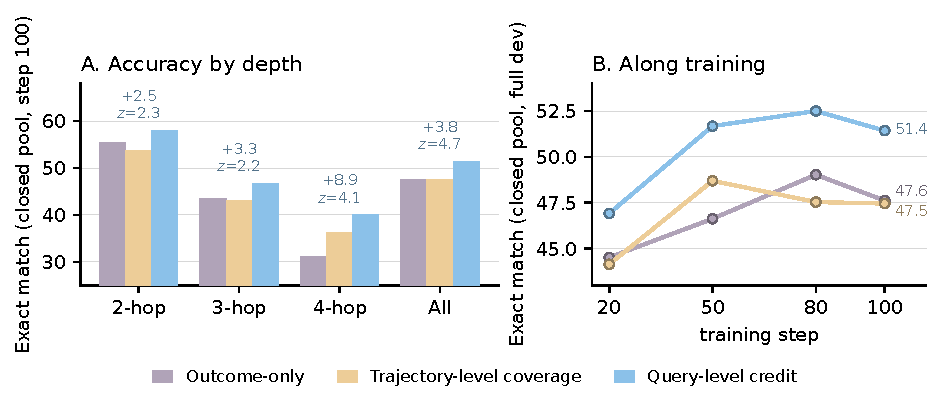
\includegraphics[width=\textwidth]{figs/fig_main_arms.pdf}
\caption{Query-level credit against outcome-only training and the
trajectory-level coverage term on closed-pool MuSiQue dev (seed 1).
(A)~Exact match by depth at step 100; annotations give query-level
credit minus outcome-only and the question-level paired McNemar $z$.
(B)~Full-dev exact match at steps 20, 50, 80, and 100. Per-hop values,
F1, final coverage, and search calls are in Table~\ref{tab:main-qc}
(Appendix~\ref{app:main-table}).}
\label{fig:arms}
\end{figure*}

\subsection{Trajectory-level coverage: four matched pairs}
\label{sec:results-pair}

Table~\ref{tab:main-pair} reports the trajectory-level coverage term
against outcome-only training over four matched pairs of runs (same
SFT initialization, schedule, data order, and rollout samples;
explicit seeds 1--3 and the default seed). Pooled over the four pairs,
4-hop exact match improves by $+3.6$ points (157:99, $z=3.62$); pooled
over the three explicit-seed pairs, by $+2.4$ (116:87, $z=2.04$). The
per-pair 4-hop differences are $+7.2$, $+4.2$, $-2.7$, and $+5.7$
(Fig.~\ref{fig:paired-seeds}). Overall EM moves by $+0.9$ ($z=2.36$;
$+0.6$, $z=1.42$, over the explicit-seed pairs), and search calls per
question are unchanged. The term breaks ties at the level of whole
trajectories and buys a deep-hop gain of this size in the training
environment; \S\ref{sec:mech-broadcast} shows what the broadcast does
at the level of turns, and \S\ref{sec:transfer-traj} what the habit it
teaches costs outside the training environment.
% 原句(v2, 6.1): "Table~\ref{tab:main-pair} reports four matched pairs of runs
% on the closed-pool MuSiQue development set: coverage-shaped RL against
% outcome-only RL ... The effect is depth-structured: pooled over the four
% pairs, $+0.2$ at two hops, $+0.6$ at three, and $+3.6$ at four. ... The
% improvement lands where \S\ref{sec:starvation} locates the all-wrong
% groups."
% 原句(v1, 单对): "Overall exact match improves by $+1.65$ points ($z=2.37$).
% ... $+7.2$ at four hops ($z=3.98$; 41 questions flip to correct against 12
% that flip to wrong). ... $-2.2$ on the easy third, $+1.8$ on the medium,
% $+5.3$ on the hard third ($z=2.72$). ... 4.70 versus 4.98 calls per question
% overall, 6.21 versus 6.56 on 4-hop questions."

\begin{table}[t]
\centering
\small
\resizebox{\columnwidth}{!}{%
\begin{tabular}{lrrrrr}
\toprule
Pair & \multicolumn{2}{c}{Overall EM} & \multicolumn{2}{c}{4-hop EM} & $\Delta$search \\
 & $\Delta$ & $z$ & $\Delta$ & $z$ & \\
\midrule
Seed 1       & $-0.25$ & $-0.31$ & $+4.20$ & $+1.99$ & $+0.10$ \\
Seed 2       & $+0.29$ & $+0.39$ & $-2.72$ & $-1.39$ & $+0.21$ \\
Seed 3       & $+1.82$ & $+2.48$ & $+5.68$ & $+2.81$ & $-0.16$ \\
Default seed & $+1.65$ & $+2.37$ & $+7.16$ & $+3.98$ & $-0.28$ \\
\midrule
Pooled, seeds 1--3 & $+0.62$ & $+1.42$ & $+2.39$ & $+2.04$ & $+0.05$ \\
Pooled, all four   & $+0.88$ & $+2.36$ & $\mathbf{+3.58}$ & $\mathbf{+3.62}$ & $-0.03$ \\
\bottomrule
\end{tabular}}
\caption{Trajectory-level coverage minus outcome-only RL across four
matched pairs (same SFT initialization, schedule, and data order;
explicit seeds 1--3 also share the sampler seed), closed-pool MuSiQue
dev (2{,}417 questions, 405 at four hops), question-level paired McNemar
$z$; $\Delta$search is the difference in search calls per question.}
\label{tab:main-pair}
\end{table}

% ---- Fig 2 占位(fig_paired_seeds.py 待写): 每对一组柱, 4hop ΔEM 与 Δsearch ----
\begin{figure}[t]
\centering
\fbox{\parbox{0.95\columnwidth}{\centering\vspace{2em}
[Figure~2 placeholder: per-pair 4-hop $\Delta$EM and $\Delta$search
for the four matched pairs of Table~\ref{tab:main-pair}, with the
pooled estimate.]\vspace{2em}}}
\caption{Per-pair deep-hop effect of the trajectory-level coverage
term. [Placeholder.]}
\label{fig:paired-seeds}
\end{figure}

\subsection{Run-level variation}
\label{sec:results-seeds}

At the run level, the trajectory-level arms of the three explicit-seed
pairs reach 47.12, 47.83, and 48.49 overall EM ($47.8 \pm 0.7$) with
4-hop EM 34.6, 33.3, and 38.0 ($35.3 \pm 2.4$); the outcome-only arms
reach 47.37, 47.54, and 46.67 ($47.2 \pm 0.5$) with 4-hop EM 30.4, 36.1,
and 32.4 ($32.9 \pm 2.9$). A separate batch of same-seed reruns of the
trajectory-level recipe, which fixes the data order and varies only
training stochasticity, spans $47.5 \pm 1.6$ (Appendix~D). Extended
training of that recipe past the fixed 100-episode endpoint reaches
50.27 EM at episode 120 and degrades beyond it (Appendix~E); the
query-level arm passes that value at step 50.

\subsection{The same-base ladder}
\label{sec:results-ladder}

Table~\ref{tab:ladder} places the result on the ladder of the same
base model in the closed pool. Closed-book answering reaches 4.8 EM; a
single retrieval of the pool's top ten paragraphs 20.8; the search
protocol alone, zero-shot, 23.8; SFT adds 12.2 points over the
zero-shot protocol (411:116, $z=12.85$); outcome-only RL adds 11.2 over
SFT ($z=22.0$); query-level credit adds 3.8 over outcome-only RL
($z=4.72$). At four hops the ladder runs
$1.7 \rightarrow 24.0 \rightarrow 13.3 \rightarrow 18.5 \rightarrow
32.9 \rightarrow 40.0$.\footnote{Ten of the pool's twenty paragraphs
cover half the pool whatever the query, which is why single-shot
retrieval scores above the zero-shot protocol at four hops.}
% 原表(v1/v2): 前三行为开卷(IRCoT 139k)口径 (4.8 / 15.4 / 29.0), SFT 行为
% SFT v3 (34.5); RL 两行 46.55/48.20 (单对) → 47.2/47.8 (种子均值)。
% 原句(v2): "outcome-only RL adds 12.7 points; coverage shaping adds 0.6 on top
% ... 1.7 → 7.9 → 10.1 → 24.9 → 32.9 → 35.3 ... the shaping term accounts for
% 2.4 points of it on the seed means and 3.6 pooled over the four matched pairs."

\begin{table}[t]
\centering
\small
\resizebox{\columnwidth}{!}{%
\begin{tabular}{lccc}
\toprule
Same policy (Qwen3.5-9B), closed pool & EM & 4-hop & F1 \\
\midrule
Closed book                       & 4.8  & 1.7  & 12.6 \\
Single-shot RAG (pool top-10)     & 20.8 & 24.0 & 28.7 \\
Search protocol, zero-shot        & 23.8 & 13.3 & 31.1 \\
SFT                               & 36.0 & 18.5 & 43.1 \\
Outcome-only RL (3 seeds)         & 47.2 & 32.9 & 55.4 \\
Trajectory-level coverage (3 seeds) & 47.8 & 35.3 & 55.9 \\
Query-level credit (seed 1)       & \textbf{51.4} & \textbf{40.0} & \textbf{59.7} \\
\bottomrule
\end{tabular}}
\caption{The same-base ladder on closed-pool MuSiQue dev. Every row is
the same base model under progressively more training; the RL rows of
seeds 1--3 are means, and the query-level row is the seed-1 run of
Table~\ref{tab:main-qc}.}
\label{tab:ladder}
\end{table}

\subsection{Comparison with external systems}
\label{sec:results-external}

Table~\ref{tab:external} places the trained policies against five
search-RL systems reproduced under one retrieval environment. On
wiki18 MuSiQue, query-level credit with continued training against the
open retriever reaches 28.55 EM against 22.09 for ReSearch, the
strongest external system (paired $z=7.80$); on HotpotQA, 48.55 against
45.00 for Search-R1 ($z=3.94$); on the 139k corpus, the
extended-training checkpoint reaches 45.64 against 32.77.

\begin{table*}[t]
\centering
\small
\begin{tabular}{lcccccc}
\toprule
 & \multicolumn{2}{c}{MuSiQue (wiki18)} & HotpotQA (wiki18) & 2Wiki (wiki18) & MuSiQue (139k) \\
System & EM & F1 & EM & EM & EM \\
\midrule
ZeroSearch~\citep{sun2026zerosearch}                     & 9.43  & 16.78 & 30.70 & --- & 11.92 \\
R1-Searcher~\citep{song2025r1searcher}                   & 15.27 & 22.88 & 39.60 & --- & 24.74 \\
StepSearch~\citep{zheng-etal-2025-stepsearch}            & 18.25 & 26.96 & 35.15 & --- & 25.49 \\
Search-R1~\citep{jin2025searchr1}                        & 20.40 & 29.50 & 45.00 & --- & 31.73 \\
ReSearch~\citep{chen2025research}                        & 22.09 & 32.43 & 44.05 & --- & 32.77 \\
\midrule
\rowcolor{shade}
Ours, query-level credit, + 50 episodes against wiki18   & \textbf{28.55} & \textbf{38.81} & \textbf{48.55} & \textbf{44.45} & 44.97 \\
Ours, extended-training checkpoint (Appendix~E)          & 26.52 & 36.90 & 47.15 & 41.75 & \textbf{45.64} \\
\bottomrule
\end{tabular}
\caption{Comparison with search-RL systems under one retrieval
environment (e5-base-v2 over wiki18 or over the 139k-paragraph MuSiQue
pool union); alias EM and F1 on full MuSiQue dev, HotpotQA and 2Wiki on
2{,}000-question subsets.}
% 表注待定(用户 2026-09-16: 先以注释保留):
% External systems are run with their released checkpoints and official
% protocols (Qwen2.5-7B); ours is Qwen3.5-9B. ReSearch and StepSearch are
% trained on MuSiQue; Search-R1 and R1-Searcher on HotpotQA. Question-level
% paired McNemar against the strongest external system on each set:
% MuSiQue vs.\ ReSearch $z=7.80$ (shaded row); HotpotQA vs.\ Search-R1 $z=3.94$. 2Wiki: external systems not yet run (6 evals);
% 139k: outcome-only step-100 arm scores 45.72 (non-paired).
\label{tab:external}
\end{table*}
        % §4 Experiments (原 §5+§6)
% ============================================================
% Section 7 — Why Does the Credit Help? (v2, 2026-09-16)
% 数据: HANDOFF §22 (K=8 修正终值: 分隔符 bug 修复后), §15 (RL 后账本 run7 s100),
%       §23 (广播诊断: 命中 turn 负优势比例), §24 (同状态重采样探针),
%       §33 (查询级信用 vs outcome-only 训练后 K=8), §20 (有据性三轴, 见 §8.1)
% v1 (2026-08-29, 修正前数字) 原句以注释保留。
% ============================================================

\section{Why Does the Credit Help?}
\label{sec:mechanism}

Section~\ref{sec:results} measures the effect of the credit on
deep-hop accuracy; this section audits what the two placements of the
evidence signal change about the groups and turns the estimator learns
from.

\subsection{Audit protocol}
\label{sec:mech-protocol}

We sample $K{=}8$ rollouts per question at the training temperature
from the SFT initialization on a stratified closed-pool question set
($n{=}160/320/319$ complete groups at 2/3/4 hops; 799 in total),
compute each rollout's coverage by the reward's definition
(Eq.~\ref{eq:coverage}), and classify every group by its answer
outcomes and its within-group coverage variation. The same audit is
repeated on trained policies: the trajectory-level arm after 100
episodes (\S\ref{sec:mech-evolution}) and the query-level and
outcome-only arms at step 100 (\S\ref{sec:mech-broken}).

\subsection{Coverage supplies ordering where outcomes are silent}
\label{sec:mech-repair}

Table~\ref{tab:repair} extends the tie ledger of
Table~\ref{tab:tie-ledger} with the repair. Under outcome-only reward,
a group is informative exactly when it is mixed: 29--44\% of groups,
and 38.2\% at four hops. Counting a group as informative when either
the answer reward or coverage discriminates, the share at four hops
rises to 88.7\%---a $\times$2.32 expansion, the largest of any depth.
The raw material behind this is the variation documented in
\S\ref{sec:starvation}: within answer-tied groups, the share whose
rollouts differ in coverage rises from 31.0\% (2-hop) through 70.4\% to
84.3\% at four hops, and all-wrong groups with coverage variation alone
make up 19.4/36.2/50.5\% of all groups. Deep tied groups are not
uniform failures; they are failures that differ in how much of the
evidence chain they recovered, and coverage converts exactly that
difference into preference.
% 原句(v1, 修正前): "... rises to 93.4\%---a $\times$2.4 expansion ... from
% 38.9\% (2-hop) through 64.8\% to 89.3\% at four hops."

\begin{table}[t]
\centering
\small
\resizebox{\columnwidth}{!}{%
\begin{tabular}{lccc}
\toprule
 & 2-hop & 3-hop & 4-hop \\
\midrule
Informative, outcome only & 29.4\% & 44.1\% & 38.2\% \\
Informative, outcome $\cup$ coverage & 48.8\% & 80.3\% & 88.7\% \\
\quad expansion & $\times$1.66 & $\times$1.82 & $\times$2.32 \\
Tied groups w/ coverage variation & 31.0\% & 70.4\% & 84.3\% \\
All-wrong groups w/ coverage variation & 19.4\% & 36.2\% & 50.5\% \\
\bottomrule
\end{tabular}}
\caption{The repair, at the SFT initialization ($K{=}8$, 799 groups):
share of groups providing any within-group ordering, before and after
adding coverage. The expansion is largest at four hops, where answer
outcomes are most often uniformly wrong.}
\label{tab:repair}
\end{table}
% 原表(v1): 56.9 / 80.3 / 93.4; ×1.94 / ×1.82 / ×2.44; 38.9 / 64.8 / 89.3.

\subsection{Coverage discriminates correctness and does not decay}
\label{sec:mech-not}

Within mixed groups, where within-group discrimination is defined,
ranking rollouts by coverage identifies the correct ones with tie-aware
AUC 0.713/0.734/0.657 at 2/3/4 hops at the SFT initialization, and
0.719/0.714/0.652 after 100 episodes of trajectory-level
training.\footnote{Average-rank tie handling; coverage values are
coarse.} Across questions, coverage against correctness reaches AUC
0.758/0.752/0.738. A quantity with this discriminative power, computed
from annotations already in the training set, is the ordering the tied
groups lack; the signal is not consumed by training. Reranking sampled
rollouts at inference by a verifier's estimate of coverage yields no
reliable gain (\S\ref{sec:placement}); the value of the signal is in
training.
% 原句(v1, 分隔符 bug 修正前, 已作废): "Coverage is a weak predictor of answer
% correctness. ... tie-aware within-group AUC of coverage against correctness
% is 0.62/0.59/0.56 at 2/3/4 hops at the SFT initialization, and lower after
% training. ... What coverage measures is \emph{progress through the annotated
% evidence chain}; its effect as a training signal is the matched comparison of
% \S\ref{sec:results}."

\subsection{Why the trajectory-level placement changes when to answer}
\label{sec:mech-broadcast}

The trajectory-level term reorders whole trajectories and broadcasts
one scalar to every turn. Replaying the reward over the $K{=}8$ audit,
a search turn that reached new gold evidence receives a negative
advantage 41.9\% of the time at the SFT initialization and 40.5\% on
the trained policy; an answer turn taken with incomplete evidence
receives a positive advantage 58.9\% and 45.1\% of the time; the
correlation between a turn's advantage and the evidence it gained is
0.04--0.25. The signal ranks trajectories but reaches no individual
step. What the policy can learn from it is the decision the trajectory
return does see---whether to answer---and the trajectory-level arm
learns exactly that: in all three retrieval environments its final
coverage equals the outcome-only arm's (81.0 vs.\ 81.2\% in the closed
pool, 78.5 vs.\ 78.6 on the 139k corpus, 46.0 vs.\ 46.2 on wiki18),
and the one measure on which the arms differ is the rate of correct
answers given from partial coverage, lower for the trajectory-level
arm in every environment ($z=-1.81$, $-2.88$, $-3.35$).

The query step carries the signal the broadcast discards. Resampling
four queries from the trained policy at a visited search state and
retrieving for each, 35--50\% of closed-pool states yield different
evidence across the four, the best and worst samples differ by
0.13--0.23 of the gold set, and the executed query is worse than one of
its own alternatives at 13--33\% of states (20--43\%, 0.07--0.13, and
12--18\% at the SFT initialization). One hundred episodes of
outcome-only training leave this variation in place. Under the dense
retriever on wiki18, 10--20\% of states show a difference and the
spread is 0.03--0.09: the policy's queries at a state tend to succeed or
fail together, which bounds what on-policy resampling can supply
there (\S\ref{sec:transfer-reach}).

\subsection{Ties are broken on the trained policy}
\label{sec:mech-broken}

Table~\ref{tab:k8-arms} audits the query-level and outcome-only arms
of seed 1 at step 100 with the same protocol. On the same 799
questions, the query-level arm has fewer all-wrong groups (32.5\% vs.\
35.5\%; at four hops 37.3\% vs.\ 42.9\%, 31 groups resolved against 13
lost, $z=2.71$) and more all-correct groups (19.4\% vs.\ 14.9\%; at four
hops 12.5\% vs.\ 7.8\%). Sampled accuracy is higher (pass@1 42.5 vs.\
38.1; at four hops 36.9 vs.\ 30.2) and so is pass@8 (67.5 vs.\ 64.5; at
four hops 62.7 vs.\ 57.1). The coverage variation inside tied groups
and its within-group AUC are the same for both arms (4-hop groups with
coverage variation 83.6 vs.\ 81.5\%; AUC 0.85 vs.\ 0.85): the signal
itself does not change with training; what changes is that the
query-level arm has used it. The ties that disappear are the
problem ties, and the ties that appear are solved ones.

\begin{table}[t]
\centering
\small
\resizebox{\columnwidth}{!}{%
\begin{tabular}{lcccc}
\toprule
$K{=}8$, step 100 & \multicolumn{2}{c}{All groups} & \multicolumn{2}{c}{4-hop} \\
 & Query credit & Outcome & Query credit & Outcome \\
\midrule
All-wrong groups (\%)   & \textbf{32.5} & 35.5 & \textbf{37.3} & 42.9 \\
All-correct groups (\%) & \textbf{19.4} & 14.9 & \textbf{12.5} & 7.8 \\
pass@1                  & \textbf{42.5} & 38.1 & \textbf{36.9} & 30.2 \\
pass@8                  & \textbf{67.5} & 64.5 & \textbf{62.7} & 57.1 \\
\bottomrule
\end{tabular}}
\caption{The tie ledger on the trained policies (seed 1, step 100, 799
closed-pool questions, temperature 0.7). Groups in which every rollout
is wrong fall and groups in which every rollout is right rise under
query-level credit; at four hops, 31 all-wrong groups of the
outcome-only arm are resolved against 13 that the query-level arm loses
($z=2.71$). At the SFT initialization the shares are 50.1\% all-wrong and
11.1\% all-correct (57.4\% and 4.4\% at four hops).}
\label{tab:k8-arms}
\end{table}

\subsection{Ties persist under the trajectory-level term}
\label{sec:mech-evolution}

Auditing the trajectory-level arm after 100 episodes, answer-tied
groups remain the majority at every depth (56.2/46.9/50.2\%), and the
informative-share expansion from coverage remains
$\times$1.61/1.69/1.87. Answer ties are a standing property of deep
search under terminal rewards, not a transient of initialization.
% 原句(v1): "([55.2]\% at four hops, [42.6]\% uniformly wrong), and the
% informative-share expansion from coverage remains [$\times$2.1]" + K6-partial 脚注。

\subsection{The mechanism, end to end}
\label{sec:mech-chain}

The audit closes the loop opened in \S\ref{sec:starvation}:
(i)~deep-hop groups are predominantly answer-tied, and with depth their
ties shift from all-right to all-wrong;
(ii)~inside those tied groups, evidence progress varies---at four hops,
in 84\% of them---and coverage discriminates correctness at AUC
0.66--0.73;
(iii)~placed on the trajectory return, that variation becomes a
ranking of whole trajectories, which the broadcast delivers to every
turn alike, so the policy learns when to answer;
(iv)~placed at the query step against the policy's own alternatives,
it becomes a per-step credit for the query that reached the evidence;
and (v)~on the trained policy, all-wrong groups fall by 5.6 points at
four hops and 4-hop accuracy rises by 8.9 (\S\ref{sec:results}).
Terminal rewards fail deep questions as a matter of arithmetic;
evidence credit at the query step repairs the arithmetic where it
fails.
% 原句(v1): "(iii) coverage converts that variation into within-group
% preferences, expanding the share of groups that provide any ordering by
% ×2.4 at four hops ...; (iv) the matched ablation shows these preferences
% causally improve deep-hop accuracy without increasing search. ... evidence
% coverage repairs the arithmetic where it fails."
      % §5 Analysis
% % ============================================================
% Section 8 — Outside the Training Environment (v2, 2026-09-16)
% 数据: HANDOFF §16 (轨迹级覆盖开放域三对配对), §20 (有据性三轴), §17/§18 (可达率),
%       §30 (查询级信用 seed 1 开放域, 严格同题配对), §31-§37 (开放续训三臂 + 闭池再训对照)
% v1 (2026-08-29, 单对结论 + "transfer is structure-dependent") 已被三对配对撤回, 原文注释在文末。
% ============================================================

\section{Outside the Training Environment}
\label{sec:transfer}

Both placements are trained in a closed pool with a lexical retriever,
where every gold document is reachable by construction. We evaluate
the trained policies zero-shot under the unified open-corpus
environment (wiki18, dense retrieval; \S\ref{sec:setup-data}) on
MuSiQue, HotpotQA, and 2WikiMultihopQA, then continue training against
that retriever.

\subsection{The trajectory-level term is a training-environment habit}
\label{sec:transfer-traj}

Table~\ref{tab:open-pairs} reports the trajectory-level coverage term
against outcome-only training over the three explicit-seed pairs on
the open corpus. Pooled, the term loses 0.8 EM on MuSiQue ($z=-2.47$),
is flat on HotpotQA ($z=-1.29$), and loses 2.75 EM on 2WikiMultihopQA
($z=-6.40$; 5.9 points at four hops, $z=-5.33$). The grounding audit
of \S\ref{sec:mech-broadcast} locates the loss: in every environment
the two arms reach the same final coverage and the same rate of
grounded correct answers, and the trajectory-level arm answers
correctly from partial coverage less often, by a margin that widens as
reachability falls ($z=-1.81$ in the closed pool, $-2.88$ on the 139k
corpus, $-3.35$ on wiki18). The arm has learned to answer only when
its evidence set is complete. In the closed pool, where the set is
always completable, the habit is neutral to slightly positive (fewer
wrong answers from full coverage at four hops, $z=-2.66$); on an open
corpus, where the set is usually not completable
(\S\ref{sec:transfer-reach}), it forfeits questions that partial
evidence would have answered.
% 原句(v1, 单对, 已撤回): "The effect survives, significantly, in two places:
% HotpotQA \emph{comparison} questions ($+4.75$, $z=+3.80$) and 2WikiMultihopQA
% overall ($+2.05$, $z=+3.01$; 4-hop $+4.52$, $z=+2.39$)---the structures whose
% questions require assembling several parallel evidence branches ..."
% 原表(v1): MuSiQue 25.69/26.40 (−1.41); Hotpot 46.40/46.30 (+0.19), bridge
% 41.13/42.19 (−1.78), comparison 67.50/62.75 (+3.80); 2Wiki 39.95/37.90 (+3.01),
% 4-hop 33.03/28.51 (+2.39)。

\begin{table}[t]
\centering
\small
\resizebox{\columnwidth}{!}{%
\begin{tabular}{lccrr}
\toprule
wiki18, three pairs & Traj.\ cov. & Outcome & $\Delta$ & pooled $z$ \\
\midrule
MuSiQue (2{,}417)  & 26.05 & 26.87 & $-0.8$ & $-2.47$ \\
\quad 4-hop        & 11.03 & 10.95 & $+0.1$ & $+0.11$ \\
HotpotQA (2{,}000) & 46.48 & 46.93 & $-0.5$ & $-1.29$ \\
\quad comparison   & 65.33 & 66.58 & $-1.3$ & $-1.59$ \\
2Wiki (2{,}000)    & 38.40 & 41.15 & $-2.8$ & $\mathbf{-6.40}$ \\
\quad 4-hop        & 29.34 & 35.22 & $-5.9$ & $\mathbf{-5.33}$ \\
\bottomrule
\end{tabular}}
\caption{Trajectory-level coverage versus outcome-only training on the
open corpus: means over the three explicit-seed pairs (step 100, no
open-corpus training), question-level paired McNemar $z$ pooled over
the pairs.}
\label{tab:open-pairs}
\end{table}

\subsection{Query-level credit on the open corpus}
\label{sec:transfer-qc}

Table~\ref{tab:open-qc} evaluates the query-level arm of seed 1 at
step 100 on the same questions as its two contrast arms. The penalty
of the trajectory-level term is absent: on 2WikiMultihopQA the
query-level arm scores 40.45 against 37.05 for the trajectory-level arm
($z=+4.46$; 34.62 vs.\ 27.15 at four hops, $z=+3.86$) and 41.25 for
the outcome-only arm ($z=-1.06$); on HotpotQA the three arms score
45.60, 45.60, and 46.50 ($z=0$ and $-1.40$). On MuSiQue the query-level
arm scores 26.35 against 25.36 and 28.01 ($z=+1.62$ and $-2.51$; the
outcome-only value is the highest of its three seeds, whose mean is
27.15), with the 4-hop lead of the closed pool carrying over (15.31
vs.\ 11.85 and 11.36, $z=+2.11$ and $+2.41$). The arm abstains far
less (5.2\% of MuSiQue questions vs.\ 12.1 and 8.5; 38.2\% of 2Wiki
4-hop questions vs.\ 56.3 and 45.9) and searches less (3.36 calls per
question vs.\ 3.78 and 3.70) at equal final coverage (45.0 vs.\ 45.5
and 46.0). The closed-pool lead does not transfer beyond four hops:
the search habit the arm learned---reach the same coverage in fewer
calls---is calibrated to the lexical pool retriever, and under the
dense retriever fewer calls reach less.

\begin{table*}[t]
\centering
\small
\begin{tabular}{lcccrr}
\toprule
wiki18, seed 1 & Query credit & Traj.\ cov. & Outcome & $z$ vs.\ traj. & $z$ vs.\ outcome \\
\midrule
MuSiQue (2{,}417)  & 26.35 & 25.36 & 28.01 & $+1.62$ & $-2.51$ \\
\quad 4-hop        & \textbf{15.31} & 11.85 & 11.36 & $+2.11$ & $+2.41$ \\
HotpotQA (2{,}000) & 45.60 & 45.60 & 46.50 & $0.00$ & $-1.40$ \\
2Wiki (2{,}000)    & 40.45 & 37.05 & 41.25 & $+4.46$ & $-1.06$ \\
\quad 4-hop        & 34.62 & 27.15 & 35.29 & $+3.86$ & $-0.33$ \\
\bottomrule
\end{tabular}
\caption{The three arms of seed 1 at step 100 on the open corpus, same
questions, question-level paired McNemar $z$ (query-level credit minus
the named arm); no arm has trained against the open retriever.}
\label{tab:open-qc}
\end{table*}

\subsection{Reachability: the bottleneck is query phrasing under the retriever}
\label{sec:transfer-reach}

Decompose success as
$P(\text{correct}) = P(\text{evidence reachable}) \times
P(\text{correct}\mid\text{reachable})$ and measure the first factor
directly (Table~\ref{tab:reach}). Against wiki18, the question itself
as a query reaches the complete gold set of 11.8/0.4/0.2\% of
MuSiQue questions at 2/3/4 hops; the official sub-questions with gold
intermediate answers substituted in, an upper bound on decomposition
quality, reach it for 43.8/24.9/15.6\%. Querying by the gold
paragraphs' titles reaches it for 80.1/62.1/62.0\%.\footnote{Title
matching across corpus versions is exact, so all reachability numbers
are lower bounds.} The paragraphs are present and the index returns
them when asked by title; natural-language sub-queries do not reach
them. On the 139k corpus the decomposition bound is 85.3/80.7/41.7\%
and the title bound 98.3/97.9/93.8\%; in the closed pool both are
100\%. The binding constraint outside the training environment is
therefore how queries are phrased for the dense retriever, which
training against that retriever can change---and it is why on-policy
resampling supplies little credit there (\S\ref{sec:mech-broadcast}):
the policy's own alternatives at a state are phrased alike.

\begin{table}[t]
\centering
\small
\resizebox{\columnwidth}{!}{%
\begin{tabular}{lccc}
\toprule
Full gold set reached, MuSiQue dev & 2-hop & 3-hop & 4-hop \\
\midrule
wiki18, question as query          & 11.8\% & 0.4\%  & 0.2\% \\
wiki18, decomposition oracle       & 43.8\% & 24.9\% & 15.6\% \\
wiki18, title oracle               & 80.1\% & 62.1\% & 62.0\% \\
139k corpus, decomposition oracle  & 85.3\% & 80.7\% & 41.7\% \\
139k corpus, title oracle          & 98.3\% & 97.9\% & 93.8\% \\
Closed pool                        & 100\%  & 100\%  & 100\% \\
\bottomrule
\end{tabular}}
\caption{Evidence reachability at top-10 dense retrieval under three
query regimes and three corpora. The decomposition oracle uses the
official sub-questions with gold intermediate answers; the title oracle
queries with the gold paragraphs' titles.}
\label{tab:reach}
\end{table}

\subsection{Continued training against the open retriever}
\label{sec:transfer-stage2}

Table~\ref{tab:stage2} continues training from the step-100
checkpoints of seed 1 for 50 episodes with wiki18 retrieval in the
loop (\S\ref{sec:setup-data}). Three arms isolate the two questions:
the outcome-only checkpoint continued with and without query-level
credit, and the query-level checkpoint continued with credit. All
three reach 28.3--28.7 EM on wiki18 MuSiQue, the highest values of
this study (the outcome-only checkpoint scores 28.01 before continuing;
the extended-training flagship of Appendix~E 26.52; the strongest
external system under the same retriever, ReSearch, 22.09). A control
that continues the same checkpoint for 30 episodes in the closed pool
instead moves the other way on every open-corpus set (MuSiQue 26.56,
$z=-2.59$; 2Wiki 38.85, $z=-3.41$): the open-corpus gain comes from the
environment, not from additional training. Transfer gains are larger
than the in-task gain: from the same checkpoint, continued training with
credit reaches 47.80 on HotpotQA and 47.00 on 2WikiMultihopQA against
46.80 and 44.30 without it ($+1.0$, $z=1.80$; $+2.7$, 132:78,
$z=3.73$), and $+0.4$ on MuSiQue ($z=0.61$). Continued training against
the open retriever lowers closed-pool EM for every arm (to 44.2--46.2
from 47.6--51.4), the mirror image of \S\ref{sec:transfer-qc}:
retrieval behaviour specializes to the retriever it is trained
against, in both directions.

\begin{table*}[t]
\centering
\small
\begin{tabular}{lccc}
\toprule
Continued on wiki18, 50 ep.\ (seed 1) & MuSiQue & HotpotQA & 2Wiki \\
\midrule
Start: outcome-only, step 100      & 28.01 & 46.50 & 41.25 \\
\quad + continued, no credit       & 28.30 & 46.80 & 44.30 \\
\quad + continued, query credit    & \textbf{28.67} & 47.80 & \textbf{47.00} \\
Start: query credit, step 100      & 26.35 & 45.60 & 40.45 \\
\quad + continued, query credit    & 28.55 & \textbf{48.55} & 44.45 \\
\midrule
Control: outcome-only, 30 ep.\ more in the closed pool & 26.56 & 45.60 & 38.85 \\
Extended-training flagship (Appendix~E), no open training & 26.52 & 47.15 & 41.75 \\
Strongest external system (wiki18)  & 22.09 & 45.00 & --- \\
\bottomrule
\end{tabular}
\caption{Continued training against the open retriever from the
step-100 checkpoints of seed 1 (alias EM on wiki18; HotpotQA and 2Wiki
on the 2{,}000-question subsets of Table~\ref{tab:open-qc}). The
external rows are ReSearch on MuSiQue and Search-R1 on HotpotQA, the
strongest of the six reproduced systems on each.}
\label{tab:stage2}
\end{table*}
      % §8 于 2026-09-16 拆入 §6.5/6.6/§7.4/附录; 原文件改名 retired_transfer.tex
% ============================================================
% Conclusion (v1, 2026-09-20)
% ============================================================
\section{Conclusion}
\label{sec:conclusion}

Group-relative RL for search agents learns only from rollouts of the
same question that differ in return, and on deep questions the answer
reward routinely does not differ: at the start of training, 57\% of
4-hop groups are uniformly wrong, and the residual ordering in such a
group favors the rollout that searched least. Gold evidence annotations
supply an ordering with content, and where that content enters the
estimator decides what the policy learns from it. Placed on the
trajectory return, it ranks whole trajectories and teaches when to
answer; placed at the query step, against the policy's own alternatives
at the same state, it credits the query that reached the evidence.
Query-level credit raises closed-pool exact match from 47.6 to 51.4 and
4-hop exact match from 31.1 to 40.0, breaks the problem ties on the
trained policy, and, after continued training against an open
retriever, yields the strongest open-corpus results among search-RL
systems reproduced under one environment. The credit is computed from
the annotations already present in multi-hop training data and the
retriever the policy searches.
     % §6
% ============================================================
% Limitations (v1, 2026-09-20; 用户: 写得概括, 不给 AI 审稿具体把柄)
% ============================================================
\section*{Limitations}

Our experiments use a single policy scale and a single family of
multi-hop training data, and the conclusions are drawn on English
Wikipedia-based benchmarks. The credit requires gold evidence
annotations at training time, which multi-hop datasets provide and many
retrieval tasks do not. Same-state sampling adds generation and
retrieval cost in proportion to $M$ at every search turn. Retrieval
behaviour learned against one retriever transfers to another only in
part, and open-corpus performance depends on the retriever the policy
is trained against.
    % Limitations (unnumbered)

\bibliography{refs}

\appendix
% ============================================================
% Appendix (started 2026-09-16). A: full three-arm table moved out of §6.1
% (user: 信息量不足以占双栏, 主文用 Fig.~\ref{fig:arms} 代替)。
% B (KL forensics), C (hyperparameters), D (same-seed reruns), E (extended
% training), F (verifier validation) 待写; 现有正文引用 Appendix~B/C/D/E/F 的
% 字母暂以文字引用, 落地后改为 \ref。
% ============================================================
\section{Three arms in the training environment: full table}
\label{app:main-table}

\begin{table*}[t]
\centering
\small
\begin{tabular}{lcccrr}
\toprule
Closed pool (dev) & Query credit & Outcome-only & Traj.\ coverage &
$z$ vs.\ outcome & $z$ vs.\ traj. \\
\midrule
EM overall (2{,}417)   & \textbf{51.43} & 47.62 & 47.46 & $+4.72$ & $+4.94$ \\
\quad 2-hop (1{,}252)  & \textbf{57.99} & 55.51 & 53.67 & $+2.32$ & $+4.02$ \\
\quad 3-hop (760)      & \textbf{46.71} & 43.42 & 43.16 & $+2.25$ & $+2.40$ \\
\quad 4-hop (405)      & \textbf{40.00} & 31.11 & 36.30 & $+4.08$ & $+1.78$ \\
F1 overall             & \textbf{59.72} & 55.16 & 55.07 & & \\
Final coverage (\%)    & \textbf{83.0}  & 81.2  & 80.4  & & \\
Full-coverage rate (\%) & \textbf{65.1} & 62.9  & 62.5  & & \\
Search calls / question & 4.31 & 4.86 & 4.93 & & \\
\bottomrule
\end{tabular}
\caption{Query-level credit against outcome-only training and the
trajectory-level coverage term: seed 1, step 100, closed-pool MuSiQue
dev, question-level paired McNemar $z$ (query-level credit minus the
named arm). The three arms share the SFT initialization, schedule, and
data order.}
\label{tab:main-qc}
\end{table*}

% 四对配对表(2026-09-16 从 §6.2 移出, 主文改用 Fig.~\ref{fig:paired-seeds})
\begin{table}[t]
\centering
\small
\resizebox{\columnwidth}{!}{%
\begin{tabular}{lrrrrr}
\toprule
Pair & \multicolumn{2}{c}{Overall EM} & \multicolumn{2}{c}{4-hop EM} & $\Delta$search \\
 & $\Delta$ & $z$ & $\Delta$ & $z$ & \\
\midrule
Seed 1       & $-0.25$ & $-0.31$ & $+4.20$ & $+1.99$ & $+0.10$ \\
Seed 2       & $+0.29$ & $+0.39$ & $-2.72$ & $-1.39$ & $+0.21$ \\
Seed 3       & $+1.82$ & $+2.48$ & $+5.68$ & $+2.81$ & $-0.16$ \\
Default seed & $+1.65$ & $+2.37$ & $+7.16$ & $+3.98$ & $-0.28$ \\
\midrule
Pooled, seeds 1--3 & $+0.62$ & $+1.42$ & $+2.39$ & $+2.04$ & $+0.05$ \\
Pooled, all four   & $+0.88$ & $+2.36$ & $\mathbf{+3.58}$ & $\mathbf{+3.62}$ & $-0.03$ \\
\bottomrule
\end{tabular}}
\caption{Trajectory-level coverage minus outcome-only RL across four
matched pairs (same SFT initialization, schedule, and data order;
explicit seeds 1--3 also share the sampler seed), closed-pool MuSiQue
dev (2{,}417 questions, 405 at four hops), question-level paired McNemar
$z$; $\Delta$search is the difference in search calls per question.}
\label{tab:main-pair}
\end{table}

% ============================================================
% Section 9 — Where Should Evidence Signals Enter the Agent? (draft v1, 2026-08-31)
% 数据: HANDOFF §6(Judge-C, 选择性预测, best-of-4)+ §9(J8 注入消融)
% 复核(2026-08-31 本窗口): rerank_results2.json = 237 题 × 4 rollouts,
%   majority 28.3 / oracle 35.0 复算吻合。
% 措辞纪律: J8 用 "no reliable improvement, trend negative"。
% ============================================================

% 2026-09-20: 整节移入附录(用户决议: 安置研究不作为贡献)
\section{Where should evidence signals enter the agent?}
\label{sec:placement}

The evidence signal of Eq.~\ref{eq:coverage} enters training at the
query step (\S\ref{sec:method-credit}) or in the trajectory return
(\S\ref{sec:method-effect}); both are one placement of a more general
resource. Evidence supervision can enter the agent at four
points: as a training reward, as an offline audit of finished
trajectories, as a runtime controller that selects among candidate
rollouts, and as an observation written into the agent's context. We
tested all four. Gold annotations exist only at training time, so the
placements that run at inference use a 4B verifier distilled from the
same annotations (held-out AUC 0.996, zero-shot 2Wiki 0.987; component
validation in Appendix~\ref{app:verifier}); on full policy rollouts it predicts answer
correctness at AUC 0.742.

\paragraph{Training reward: works.} As a reward the signal produces
the deep-hop gains of \S\ref{sec:results}, through the query-step
credit of \S\ref{sec:method-credit} and, more weakly, through the
trajectory ranking of \S\ref{sec:method-effect}
(\S\ref{sec:mechanism}).

\paragraph{Offline audit: works.} Scoring finished trajectories,
evidence coverage supports selective
prediction~\citep{geifman2017selective}: on a stratified audit set of
600 trajectories with 49\% base accuracy, answering only the 5\%
ranked most-covered yields 79\% accuracy, and the 10\% level yields
63\%. The subset whose plan is fully resolved---5.8\% of
questions---is 82\% correct.

\paragraph{Runtime control: fails.} Reranking four sampled rollouts
per question by verifier-scored evidence coverage yields 26.6--27.0
EM across every scoring strategy on a 237-question audit
set---below majority vote at 28.3, with the best-of-4 oracle at
35.0. The trajectories explain the failure: even correct rollouts
fill their declared plan slots in order at rates of only
60/19/7.5/2.4\% for slots one through four, so plan-anchored
evidence scoring systematically undervalues rollouts that reach the
answer off-plan.

\paragraph{Injected observation: fails.} From a common checkpoint,
two variants trained in the same window under identical guard criteria:
one receives a verifier-computed slot-status line in every
observation, one does not. At the last common evaluation step the
injected variant scores 46.71 versus 47.83 for the control on the full
dev set ($z=-1.80$; 99:126): no reliable improvement, and the trend
is negative. The dynamics show why. Injection costs $-4.8$ points at
twenty episodes, and the policy then adapts back to parity---it
learns to ignore the extra line rather than exploit it. The budget
line already present in the observation carries the
stopping-relevant information, and the verifier's conservative bias
(the plan--path misalignment above) leaves little marginal signal to
use.

\paragraph{Reading.} The pattern follows from what the signal
measures. Coverage separates correct from incorrect rollouts within a
group at AUC 0.66--0.73 (\S\ref{sec:mech-not}); at inference only a
verifier's estimate of it is available. Progress supervision pays where
% 原句: "Coverage quantifies evidence progress, not answer correctness
% (\S\ref{sec:mech-not})."
it reorders learning or stratifies risk after the fact; it has no
purchase where a single decision must be steered at inference, and
the policy's divergence between declared plans and executed paths
degrades every plan-anchored use. Evidence supervision is
placement-sensitive: the same deterministic signal, unchanged, moves
from decisive to useless as it moves across these four entry points.
      % 附录: 安置研究 (2026-09-20 自正文 §9 移入)

\end{document}
